%!TEX root = ./template-skripsi.tex

\subsection{Sprint 7 Report}
Berikut merupakan report dari sprint ke-7 yang dilakukan pada tanggal 6 juni - 12 juni 2022.

\begin{table}[H]
	\caption{\textit{Sprint-7 backlog}}
	\label{sprint7_backlog}
	\begin{tabular}{@{} |p{0.5cm}|p{5cm}|p{5cm}|p{2cm}| @{}}
		\hline
		\textbf{No} & \textbf{\textit{Story}} & \textbf{\textit{Task}} & \textbf{\textit{Status}} \\
		\hline
		1 & \multirow{3}{5cm}{Create, Read, Updte, dan Delete untuk Pencatatan perpindahan ikan} & Membarui desain database  & Completed\\
		\cline{1-1}\cline{3-4}
		2 & & Menambahkan routes API & Completed\\
		\cline{1-1}\cline{3-4}
		3 & & Implementasi controller entry perpindahan ikan & Completed\\
		\cline{1-1}\cline{3-4}
		4 & & Implementasi controller fetch list perpindahan ikan & Completed\\
		\cline{1-1}\cline{3-4}
		5 & & Implementasi controller edit perpindahan ikan & Completed\\
		\cline{1-1}\cline{3-4}
		6 & & Implementasi controller delete perpindahan ikan & Completed\\
		\cline{1-1}\cline{3-4}
		7 & & Implementasi controller fetch perpindahan ikan dengan id& Completed\\
		\cline{1-1}\cline{3-4}
		8 & & Membuat view rekap perpindahan ikan & Completed\\
		\cline{1-1}\cline{3-4}
		\hline
	\end{tabular}
\end{table}

\begin{enumerate}[1.]

\item \textbf{Membarui desain database}

\begin{figure}[H]
	\centering
	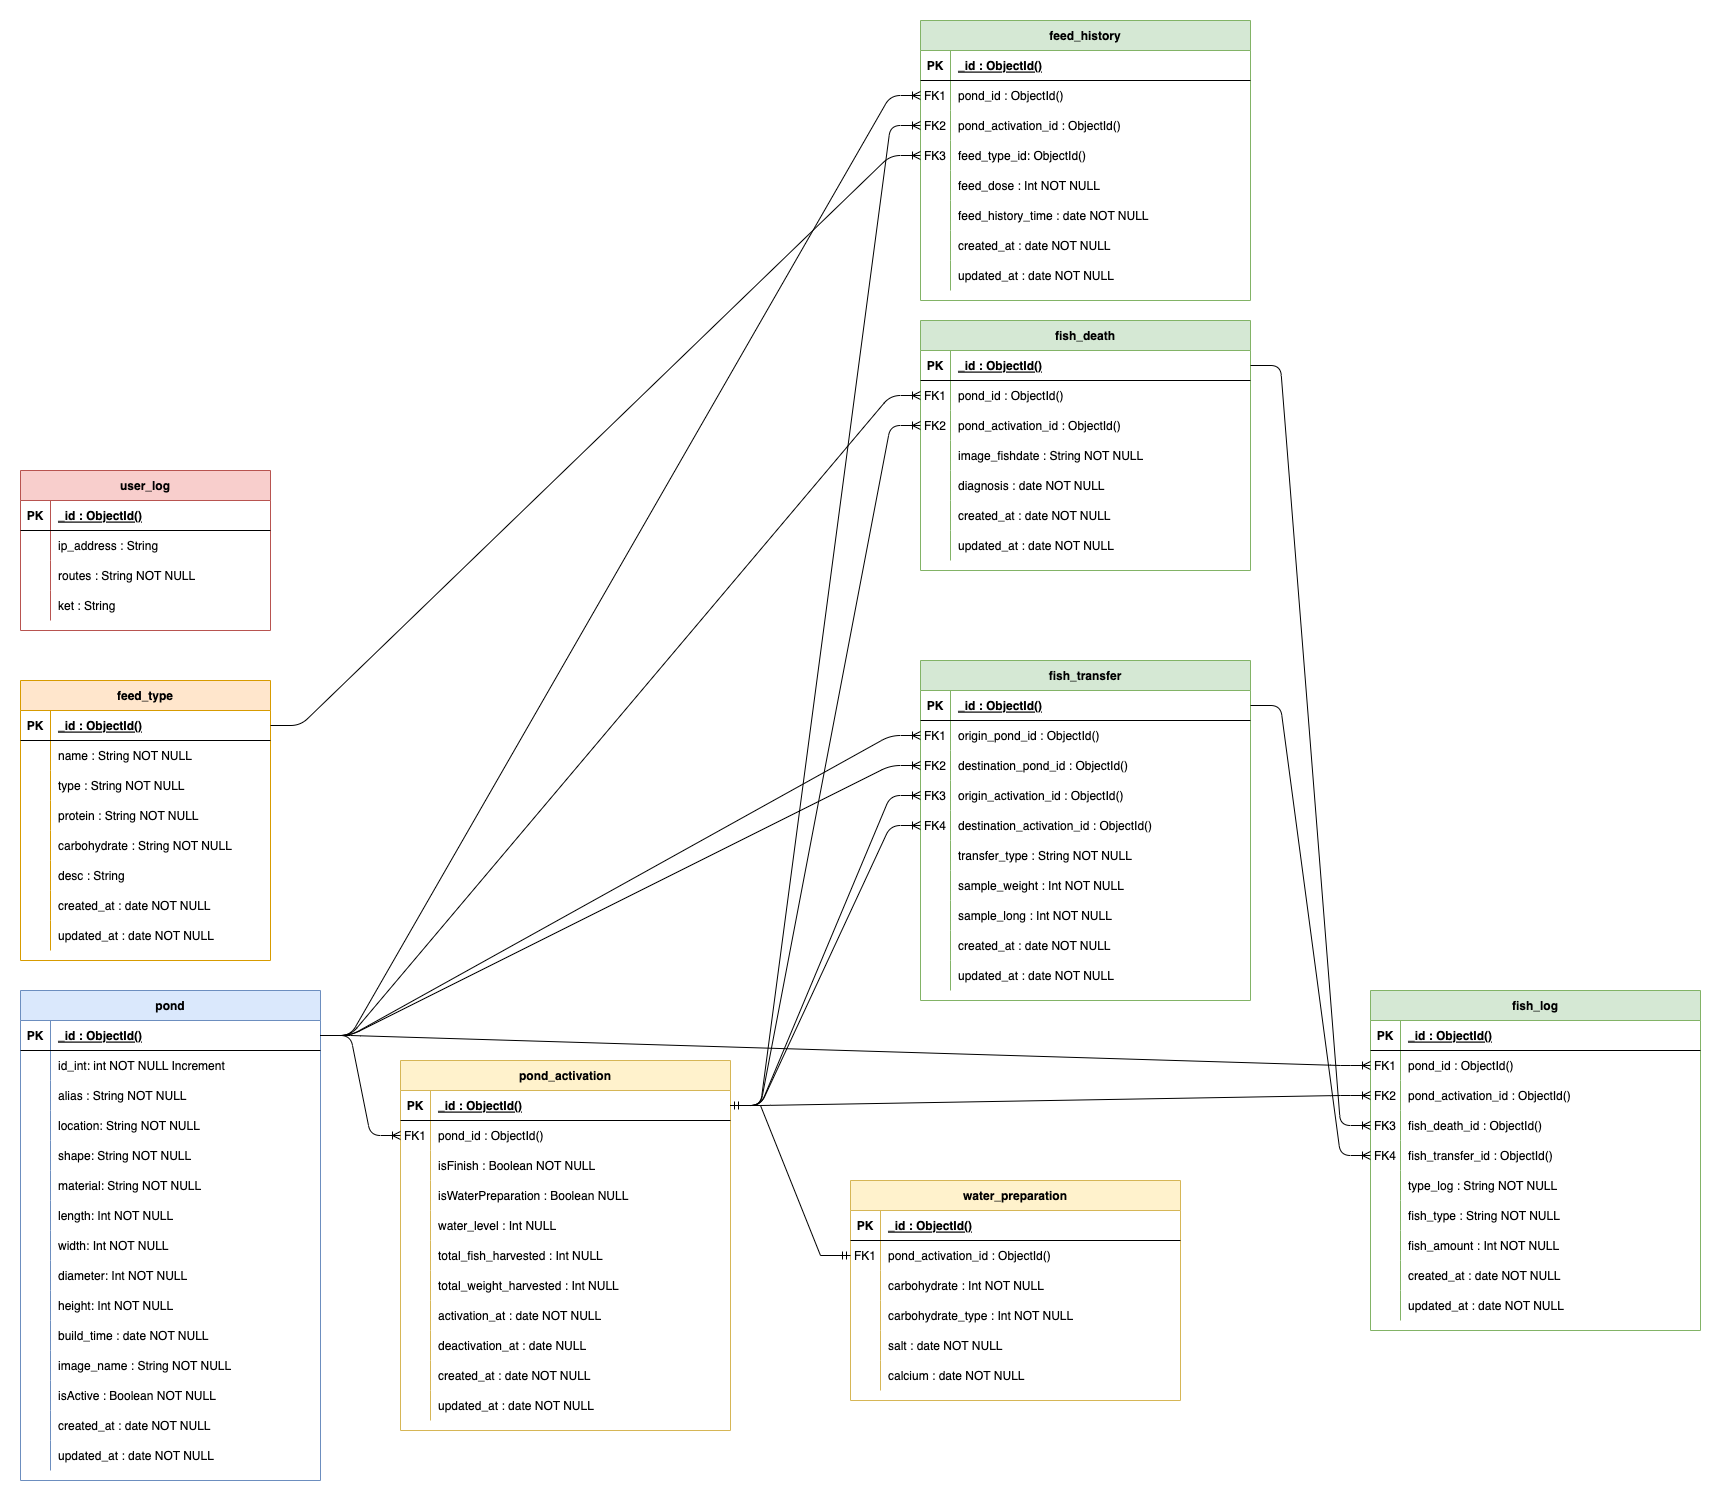
\includegraphics[height=0.7\textwidth]{gambar/Sprint07/diagram database/database}
	\caption{ERD Database Sprint-7}
	\label{fig:database_sprint7}
\end{figure}

Dengan berubahnya desain database diperlukan juga penambahan model pada source code, berikut perubahan pada source code model.

\begin{lstlisting}
# fishapi/database/model.py

class FishTransfer(db.Document):
    origin_pond_id = db.ReferenceField(Pond, required=True)
    destination_pond_id = db.ReferenceField(Pond, required=True)
    origin_activation_id = db.ReferenceField(PondActivation, required=True)
    destination_activation_id = db.ReferenceField(
        PondActivation, required=True)
    transfer_type = db.StringField(required=True)
    sample_weight = db.IntField(required=True)
    sample_long = db.IntField(required=True)
    created_at = db.DateTimeField(default=datetime.datetime.now)
    updated_at = db.DateTimeField(default=datetime.datetime.now)
\end{lstlisting}



\item \textbf{Menambahkan routes API}

\begin{lstlisting}
# fishapi/resource/routes.py

 # fish transfer
    api.add_resource(FishTransfersApi, '/api/fishtransfer')
    api.add_resource(FishTransferApi, '/api/fishtransfer/<id>')
\end{lstlisting}




\item \textbf{Implementasi controller entry perpindahan ikan}

Implementasi controller API entry perpindahan ikan, berikut merupakan perubahan source code controller API entry perpindahan ikan.

\begin{lstlisting}
# fishapi/database/fishtransfer.py

class FishTransfersApi(Resource):
    def post(self):
        try:
            origin_pond_id = request.form.get("origin_pond_id", None)
            origin_pond = Pond.objects.get(id=origin_pond_id)
            if origin_pond.isActive == False:
                response = {"message": "status pond is not active"}
                response = json.dumps(response, default=str)
                return Response(response, mimetype="application/json", status=400)
            origin_activation = PondActivation.objects(
                pond_id=origin_pond_id, isFinish=False).order_by('-activated_at').first()
            destination_pond_id = request.form.get("destination_pond_id", None)
            destination_pond = Pond.objects.get(id=destination_pond_id)
            if destination_pond.isActive == False:
                response = {"message": "status pond is not active"}
                response = json.dumps(response, default=str)
                return Response(response, mimetype="application/json", status=400)
            destination_activation = PondActivation.objects(
                pond_id=destination_pond_id, isFinish=False).order_by('-activated_at').first()
            fish_grading_id = request.form.get("fish_grading_id", None)
            transfer_type = request.form.get("transfer_type", None)
            transfer_method = request.form.get("transfer_method", None)
            sample_weight = request.form.get("sample_weight", None)
            sample_long = request.form.get("sample_long", None)
            fishes = request.form.get("fish", "[]")
            fishes = json.loads(fishes)
            if len(fishes) < 1:
                response = {"message": "There is no fish"}
                response = json.dumps(response, default=str)
                return Response(response, mimetype="application/json", status=400)
            # if transfer method is "kering" deactived pond
            if transfer_method == "kering":
                # update activation
                pond_deactivation_data = {
                    "isFinish": True,
                    "total_fish_harvested": request.form.get("total_fish_harvested", None),
                    "total_weight_harvested": request.form.get("total_weight_harvested", None),
                    "deactivated_at": request.form.get("deactivated_at", datetime.datetime.now()),
                    "deactivated_description": "sortir kering"
                }
                origin_activation.update(**pond_deactivation_data)
                pond.update(**{"isActive": False})
            # update fish grading [optional]
            if fish_grading_id and transfer_method != "kering":
                # pengecekan fish_grading
                fish_grading = FishGrading.objects.get(id=fish_grading_id)
                # update fishgrading
                if transfer_type == "oversized_transfer":
                    fish_grading.update(**{"isOversizeTransferred": True})
                else:
                    fish_grading.update(**{"isUndersizeTransferred": True})
            # save data
            data = {
                "origin_pond_id": origin_pond_id,
                "destination_pond_id": destination_pond_id,
                "origin_activation_id": origin_activation.id,
                "destination_activation_id": destination_activation.id,
                "fish_grading_id": None if transfer_method == "kering" else fish_grading_id,
                "transfer_type": None if transfer_method == "kering" else transfer_type,
                "transfer_method": transfer_method,
                "transfer_type": transfer_type,
                "sample_weight": sample_weight,
                "sample_long": sample_long
            }
            fish_transfer = FishTransfer(**data).save()
            # transfer out
            for fish in fishes:
                # save fish log
                data = {
                    "pond_id": origin_pond_id,
                    "pond_activation_id": origin_activation.id,
                    "fish_transfer_id": fish_transfer.id,
                    "type_log": "transfer_out",
                    "fish_type": fish['type'],
                    "fish_amount": fish['amount'] * -1
                }
                fishlog = FishLog(**data).save()
            # transfer in
            for fish in fishes:
                # save fish log
                data = {
                    "pond_id": destination_pond_id,
                    "pond_activation_id": destination_activation.id,
                    "fish_transfer_id": fish_transfer.id,
                    "type_log": "transfer_in",
                    "fish_type": fish['type'],
                    "fish_amount": fish['amount']
                }
                fishlog = FishLog(**data).save()
            response = {"message": "success add fishdeath"}
            response = json.dumps(response, default=str)
            return Response(response, mimetype="application/json", status=200)
        except Exception as e:
            response = {"message": str(e)}
            response = json.dumps(response, default=str)
            return Response(response, mimetype="application/json", status=400)
\end{lstlisting}

Pada awalnya, kode tersebut melakukan beberapa hal berikut:

\begin{enumerate}[(1)]
\item Menerima data dari permintaan POST yang dikirim oleh klien.
\item Memeriksa status kolam asal (origin\_pond) menggunakan origin\_pond\_id. Jika kolam tidak aktif, maka akan dikembalikan respons dengan pesan "status kolam tidak aktif".
\item Mengambil aktivasi kolam asal yang belum selesai (isFinish=False) berdasarkan origin\_pond\_id dan diurutkan berdasarkan waktu aktivasi terakhir (activated\_at).
\item Memeriksa status kolam tujuan (destination\_pond) menggunakan destination\_pond\_id. Jika kolam tidak aktif, maka akan dikembalikan respons dengan pesan "status kolam tidak aktif".
\item Mengambil aktivasi kolam tujuan yang belum selesai (isFinish=False) berdasarkan destination\_pond\_id dan diurutkan berdasarkan waktu aktivasi terakhir (activated\_at).
\end{enumerate}

Selanjutnya, kode tersebut melakukan beberapa tugas lainnya:

\begin{enumerate}[(1)]
\item Mengambil data seperti fish\_grading\_id, transfer\_type, transfer\_method, sample\_weight, sample\_long, dan fishes dari permintaan POST.
\item Memeriksa apakah terdapat ikan dalam fishes. Jika tidak ada ikan, maka akan dikembalikan respons dengan pesan "Tidak ada ikan".
\item Jika metode transfer adalah "kering", maka akan dilakukan deaktivasi kolam asal. Data aktivasi kolam akan diperbarui dengan mengatur isFinish menjadi True dan mengisi informasi terkait seperti jumlah ikan yang dipanen, bobot total yang dipanen, waktu deaktivasi, dan deskripsi deaktivasi.
\item Jika terdapat fish\_grading\_id dan metode transfer bukan "kering", maka akan dilakukan pembaruan pada penilaian ikan. Jika transfer\_type adalah "oversized\_transfer", maka isOversizeTransferred akan diatur sebagai True. Jika tidak, isUndersizeTransferred akan diatur sebagai True.
\item Data yang diperoleh akan disimpan dalam variabel data untuk digunakan nanti.
\item Dilakukan penyimpanan data transfer ikan menggunakan model FishTransfer.
\item Dilakukan transfer ikan keluar (transfer out) dan transfer ikan masuk (transfer in) untuk setiap ikan dalam fishes. Untuk setiap ikan, data log ikan akan disimpan menggunakan model FishLog.
\item Setelah semua operasi selesai, respons dengan pesan "success add fishdeath" akan dikirim kembali kepada klien.
\end{enumerate}

Jika terjadi kesalahan selama proses tersebut, akan ditangkap oleh blok except dan respons dengan pesan kesalahan yang sesuai akan dikirim kembali kepada klien.

Berikut merupakan form untuk entry perpindahan ikan antar kolam.

\begin{longtable}{| l | p{5cm} | p{5cm} |}
\caption{Form entry kematian ikan.\label{table:form_entry_kematian_ikan}}\\

\hline
\multicolumn{1}{|c|}{\textbf{Form}} & \multicolumn{1}{|c|}{\textbf{Jenis Data}} & \multicolumn{1}{|c|}{\textbf{Deskripsi}}\\
\hline
\endfirsthead

\hline
\multicolumn{3}{|c|}{Lanjutan Tabel \ref{table:form_entry_kematian_ikan}}\\
\hline
\multicolumn{1}{|c|}{\textbf{Form}} & \multicolumn{1}{|c|}{\textbf{Jenis Data}} & \multicolumn{1}{|c|}{\textbf{Deskripsi}}\\
\hline
\endhead

                                          

origin\_pond\_id         & REQUIRED STRING                                                                                                                                             & id kolam asal ikan yang akan di transfer                                                                                                                                                      \\ \hline
destination\_pond\_id    & REQUIRED STRING                                                                                                                                             & id kolam tujuan ikan yang akan di transfer                                                                                                                                                    \\ \hline
fish                     & REQUIRED JSON FISH TYPE: {[}"nila hitam", "nila merah", "lele", "patin", "mas",{]} Ex: {[}\{"type": "lele","amount": 5\},\{"type": "patin","amount": 9\}{]} & tipe dan banyak ikan                                                                                                                                                                          \\ \hline
transfer\_method         & REQUIRED STRING TYPE: {[}"kering","basah"{]}                                                                                                                & metode transfer ikan, jika kering kolam akan dianggap panen sekaligus                                                                                                                         \\ \hline
sample\_weight           & REQUIRED INT                                                                                                                                                & sample berat ikan yang dipindahkan                                                                                                                                                            \\ \hline
sample\_long             & REQUIRED INT                                                                                                                                                & sample panjang ikan yang dipindahkan                                                                                                                                                          \\ \hline
transfer\_type           & REQUIRED STRING TYPE; {[}"oversized\_transfer", "undersized\_transfer"{]}                                                                                    & tipe transfer, "oversized\_transfer" adalah perpindahan yang dilakukan karena ikan terlalu besar dari pada ikan yang ada di kolam asal, sedangkan "undersized\_transfer" adalah kebalikannya" \\ \hline
total\_fish\_harvested   & REQUIRED IF "transfer\_method" IS "kering" INT                                                                                                              & total ikan yang dipanen bila "transfer\_method" adalah "kering"                                                                                                                               \\ \hline
total\_weight\_harvested & REQUIRED IF "transfer\_method" IS "kering" INT                                                                                                              & total berat ikan yang dipanen bila "transfer\_method" adalah "kering"                                                                                                                         \\ \hline

\end{longtable}


Berikut adalah penjelasan rinci dari setiap kolom dalam tabel tersebut:

\begin{enumerate}
\item "origin\_pond\_id": Variabel yang diperlukan, berupa string yang mengidentifikasi ID kolam asal ikan yang akan ditransfer.
\item "destination\_pond\_id": Variabel yang diperlukan, berupa string yang mengidentifikasi ID kolam tujuan ikan yang akan ditransfer.
\item "fish": Variabel yang diperlukan, berupa JSON yang mengandung tipe dan jumlah ikan yang akan ditransfer. Contoh format JSON: [{"type": "lele", "amount": 5}, {"type": "patin", "amount": 9}]. Menggambarkan jenis dan jumlah ikan yang akan ditransfer.
\item "transfer\_method": Variabel yang diperlukan, berupa string yang mengindikasikan metode transfer ikan. Jika nilainya "kering", itu berarti kolam akan dianggap sedang dipanen secara keseluruhan. Jika nilainya "basah", maka transfer akan dilakukan dengan metode lain.
\item "sample\_weight": Variabel yang diperlukan, berupa bilangan bulat (integer) yang mewakili berat sampel ikan yang akan ditransfer.
\item "sample\_long": Variabel yang diperlukan, berupa bilangan bulat (integer) yang mewakili panjang sampel ikan yang akan ditransfer.
\item "transfer\_type": Variabel yang diperlukan, berupa string yang menentukan tipe transfer. Nilainya bisa "oversized\_transfer" jika ikan yang ditransfer terlalu besar dibandingkan dengan ikan di kolam asal, atau "undersized\_transfer" jika ikan yang ditransfer terlalu kecil dibandingkan dengan ikan di kolam asal.
\item "total\_fish\_harvested": Variabel yang diperlukan jika "transfer\_method" adalah "kering", berupa bilangan bulat (integer) yang mewakili total jumlah ikan yang dipanen.
\item "total\_weight\_harvested": Variabel yang diperlukan jika "transfer\_method" adalah "kering", berupa bilangan bulat (integer) yang mewakili total berat ikan yang dipanen.
\end{enumerate}

Berikut merupakan hasil test request dari API entry perpindahan ikan antar kolam.

cURL:

\begin{lstlisting}
curl --location 'http://jft.web.id/fishapi/api/fishtransfer' \
--form 'origin_pond_id="62a62163e445ffb9c5f746f3"' \
--form 'destination_pond_id="625d7033a9a73e090c65cda2"' \
--form 'fish="[{\"type\": \"lele\",\"amount\": 30},{\"type\": \"patin\",\"amount\": 10}]"' \
--form 'sample_weight="20"' \
--form 'sample_long="50"'
\end{lstlisting}

response json:

\begin{lstlisting}
{
  "message": "success add fishtransfer"
}
\end{lstlisting}




\item \textbf{Implementasi API fetch list perpindahan ikan}

Implementasi controller API fetch list perpindahan ikan, berikut merupakan source code controller API fetch list perpindahan ikan.

\begin{lstlisting}
# fishapi/resource/fishtransfer.py

def get(self):
        try:
            pipeline = [
                {'$lookup': {
                    'from': 'pond',
                    'let': {"pondid": "$origin_pond_id"},
                    'pipeline': [
                        {'$match': {
                            '$expr': {'$eq': ['$_id', '$$pondid']}}},
                        {"$project": {
                            "created_at": 0,
                            "updated_at": 0,
                        }}
                    ],
                    'as': 'origin_pond'
                }},
                {'$lookup': {
                    'from': 'pond',
                    'let': {"pondid": "$destination_pond_id"},
                    'pipeline': [
                        {'$match': {
                            '$expr': {'$eq': ['$_id', '$$pondid']}}},
                        {"$project": {
                            "created_at": 0,
                            "updated_at": 0,
                        }}
                    ],
                    'as': 'destination_pond'
                }},
                {"$addFields": {
                    "origin_pond": {"$first": "$origin_pond"},
                    "destination_pond": {"$first": "$destination_pond"},
                }},
                {'$lookup': {
                    'from': 'fish_log',
                    'let': {"fish_transfer_id": "$_id"},
                    'pipeline': [
                        {'$match': {
                            '$expr': {'$and': [
                                {'$eq': ['$fish_transfer_id',
                                         '$$fish_transfer_id']},
                                {'$eq': ['$type_log',
                                         'transfer_out']},
                            ]}
                        }},
                        {"$project": {
                            "created_at": 0,
                            "updated_at": 0,
                        }}
                    ],
                    'as': 'fish'
                }},
                {"$project": {
                    "updated_at": 0,
                    "created_at": 0,
                }}

            ]
            fishtransfers = FishTransfer.objects.aggregate(pipeline)
            fishtransfers = list(fishtransfers)
            response = json.dumps(fishtransfers, default=str)
            return Response(response, mimetype="application/json", status=200)
        except Exception as e:
            response = {"message": str(e)}
            response = json.dumps(response, default=str)
            return Response(response, mimetype="application/json", status=400)
\end{lstlisting}


Kode diatas adalah sebuah fungsi yang mengambil data transfer ikan dari database. Fungsi ini menggunakan operasi agregasi MongoDB untuk melakukan penggabungan (lookup) antara koleksi "fish\_transfer" dengan koleksi "pond" dan "fish\_log" untuk mengambil data terkait.

Pertama, fungsi ini mendefinisikan sebuah pipeline yang berisi serangkaian operasi agregasi. Operasi pertama adalah \$lookup yang menghubungkan koleksi "fish\_transfer" dengan koleksi "pond" berdasarkan origin\_pond\_id. Hasil penggabungan ini disimpan dalam field origin\_pond. Operasi yang sama juga dilakukan untuk menggabungkan koleksi "fish\_transfer" dengan koleksi "pond" berdasarkan destination\_pond\_id, dan hasilnya disimpan dalam field destination\_pond.

Selanjutnya, dilakukan operasi \$addFields untuk mengambil nilai pertama dari field origin\_pond dan destination\_pond, dan menyimpannya dalam field yang sama. Setelah itu, dilakukan \$lookup kembali untuk menggabungkan koleksi "fish\_transfer" dengan koleksi "fish\_log" berdasarkan \_id dari transfer ikan. Hasil penggabungan ini disimpan dalam field fish.

Akhirnya, dilakukan operasi \$project untuk menghilangkan field updated\_at dan created\_at dari hasil akhir. Seluruh pipeline diterapkan pada koleksi "fish\_transfer" menggunakan fungsi aggregate, dan hasilnya dikonversi menjadi daftar Python. Data tersebut kemudian diubah menjadi format JSON menggunakan json.dumps, dan dikembalikan sebagai respons dengan tipe konten "application/json" dan kode status 200.

Jika terjadi kesalahan selama proses, pengecualian akan ditangkap dan sebuah respons JSON yang berisi pesan kesalahan akan dikirim dengan tipe konten "application/json" dan kode status 400.

Berikut merupakan hasil test request dari API fetch list perpindahan ikan antar kolam.

cURL:

\begin{lstlisting}
curl --location 'http://jft.web.id/fishapi/api/fishtransfer'
\end{lstlisting}

response json:

\begin{lstlisting}
[
  {
    "_id": "62d564220d9bde3218b4951b",
    "origin_pond_id": "62a62163e445ffb9c5f746f3",
    "destination_pond_id": "625d7033a9a73e090c65cda2",
    "origin_activation_id": "62d3f2180d7265ab60f9cb83",
    "destination_activation_id": "62d562e676d3a668927c511f",
    "sample_weight": 20,
    "sample_long": 50,
    "origin_pond": {
      "_id": "62a62163e445ffb9c5f746f3",
      "id_int": 4,
      "alias": "charlie",
      "location": "blok 2",
      "shape": "persegi",
      "material": "tanah",
      "length": 5,
      "width": 3,
      "diameter": 0,
      "height": 1,
      "build_at": "2022-06-13 00:24:51.473000",
      "image_name": "kolam_1656312365.jpeg",
      "isActive": true
    },
    "destination_pond": {
      "_id": "625d7033a9a73e090c65cda2",
      "id_int": 3,
      "alias": "beta",
      "location": "blok 10",
      "shape": "persegi",
      "material": "terpal",
      "length": 8,
      "width": 4,
      "diameter": 0,
      "height": 1,
      "build_at": "2022-04-18 21:05:39.608000",
      "image_name": "default.jpg",
      "isActive": true
    },
    "fish": [
      {
        "_id": "62d564220d9bde3218b4951c",
        "pond_id": "62a62163e445ffb9c5f746f3",
        "pond_activation_id": "62d3f2180d7265ab60f9cb83",
        "fish_transfer_id": "62d564220d9bde3218b4951b",
        "type_log": "transfer_out",
        "fish_type": "lele",
        "fish_amount": -20
      },
      {
        "_id": "62d564220d9bde3218b4951d",
        "pond_id": "62a62163e445ffb9c5f746f3",
        "pond_activation_id": "62d3f2180d7265ab60f9cb83",
        "fish_transfer_id": "62d564220d9bde3218b4951b",
        "type_log": "transfer_out",
        "fish_type": "patin",
        "fish_amount": -20
      }
    ]
  },
  {
    "_id": "62d57d8b08d03adbb8cff042",
    "origin_pond_id": "62a62163e445ffb9c5f746f3",
    "destination_pond_id": "625d7033a9a73e090c65cda2",
    "origin_activation_id": "62d3f2180d7265ab60f9cb83",
    "destination_activation_id": "62d562e676d3a668927c511f",
    "sample_weight": 20,
    "sample_long": 50,
    "origin_pond": {
      "_id": "62a62163e445ffb9c5f746f3",
      "id_int": 4,
      "alias": "charlie",
      "location": "blok 2",
      "shape": "persegi",
      "material": "tanah",
      "length": 5,
      "width": 3,
      "diameter": 0,
      "height": 1,
      "build_at": "2022-06-13 00:24:51.473000",
      "image_name": "kolam_1656312365.jpeg",
      "isActive": true
    },
    "destination_pond": {
      "_id": "625d7033a9a73e090c65cda2",
      "id_int": 3,
      "alias": "beta",
      "location": "blok 10",
      "shape": "persegi",
      "material": "terpal",
      "length": 8,
      "width": 4,
      "diameter": 0,
      "height": 1,
      "build_at": "2022-04-18 21:05:39.608000",
      "image_name": "default.jpg",
      "isActive": true
    },
    "fish": [
      {
        "_id": "62d57d8b08d03adbb8cff043",
        "pond_id": "62a62163e445ffb9c5f746f3",
        "pond_activation_id": "62d3f2180d7265ab60f9cb83",
        "fish_transfer_id": "62d57d8b08d03adbb8cff042",
        "type_log": "transfer_out",
        "fish_type": "lele",
        "fish_amount": -30
      },
      {
        "_id": "62d57d8b08d03adbb8cff044",
        "pond_id": "62a62163e445ffb9c5f746f3",
        "pond_activation_id": "62d3f2180d7265ab60f9cb83",
        "fish_transfer_id": "62d57d8b08d03adbb8cff042",
        "type_log": "transfer_out",
        "fish_type": "patin",
        "fish_amount": -10
      }
    ]
  }
]
\end{lstlisting}



\item \textbf{Implementasi API edit perpindahan ikan}

Implementasi controller API edit perpindahan ikan, berikut merupakan perubahan source code controller API edit perpindahan ikan.

\begin{lstlisting}
# fishapi/database/fishtransfer.py

def put(self, id):
        try:
            body = request.form.to_dict(flat=True)
            FishDeath.objects.get(id=id).update(**body)
            response = {"message": "success change data fish death", "id": id}
            response = json.dumps(response, default=str)
            return Response(response, mimetype="application/json", status=200)
        except Exception as e:
            response = {"message": str(e)}
            response = json.dumps(response, default=str)
            return Response(response, mimetype="application/json", status=400)
\end{lstlisting}

Kode di atas adalah sebuah fungsi yang digunakan untuk mengubah data kematian ikan dalam database. Fungsi ini menerima parameter id yang merupakan ID unik dari data kematian ikan yang ingin diubah.

Pada awalnya, fungsi ini mengambil data dari permintaan (request) dalam bentuk formulir dan mengonversinya menjadi kamus (dictionary) menggunakan metode to\_dict(flat=True). Kamus ini kemudian disimpan dalam variabel body.

Selanjutnya, fungsi ini menggunakan metode get() dari model FishDeath untuk mendapatkan objek kematian ikan berdasarkan ID yang diberikan. Setelah itu, metode update() dipanggil pada objek tersebut dengan meneruskan body sebagai argumen. Ini akan mengubah nilai-nilai properti objek sesuai dengan nilai-nilai dalam kamus body.

Setelah berhasil mengubah data kematian ikan, fungsi ini mengembalikan respons sukses dalam format JSON. Pesan respons berisi informasi bahwa data kematian ikan telah berhasil diubah, beserta ID dari data yang telah diubah. Pesan respons kemudian diubah menjadi bentuk JSON menggunakan json.dumps, dan dikembalikan sebagai respons dengan tipe konten "application/json" dan kode status 200.

Namun, jika terjadi kesalahan selama proses, pengecualian akan ditangkap dan sebuah respons JSON yang berisi pesan kesalahan akan dikirim. Pesan kesalahan akan menampilkan detail dari pengecualian yang terjadi. Respons JSON tersebut juga dikembalikan dengan tipe konten "application/json" dan kode status 400.

Berikut merupakan hasil test request dari API edit perpindahan ikan antar kolam.

cURL:

\begin{lstlisting}
curl --location -g --request PUT 'http://jft.web.id/fishapi/api/fishtransfer/{fishtransfer_id}' \
--form 'sample_weight="20"' \
\end{lstlisting}

response json:

\begin{lstlisting}
{
  "message": "success change data fish transfer",
  "id": "62b9adfa793e0f39dbaa1739"
}
\end{lstlisting}



\item \textbf{Implementasi API delete perpindahan ikan}

Implementasi controller API delete perpindahan ikan, berikut merupakan perubahan source code controller API delete perpindahan ikan.

\begin{lstlisting}
# fishapi/database/fishtransfer.py

def delete(self, id):
        try:
            fishtransfer = FishTransfer.objects.get(id=id)
            # delete fish
            fishes = FishLog.objects.aggregate([
                {'$match': {
                    '$expr': {'$eq': ['$fish_transfer_id', {'$toObjectId': id}]}}},
            ])
            for fish in fishes:
                fishlog = FishLog.objects.get(id=fish['_id'])
                fishlog.delete()
            # delete data
            fishtransfer.delete()
            response = {"message": "success delete fishtransfer"}
            response = json.dumps(response, default=str)
            return Response(response, mimetype="application/json", status=200)
        except Exception as e:
            response = {"message": str(e)}
            response = json.dumps(response, default=str)
            return Response(response, mimetype="application/json", status=400)
\end{lstlisting}

Kode di atas merupakan sebuah fungsi yang digunakan untuk menghapus data transfer ikan dari database. Fungsi ini menerima parameter id yang merupakan ID unik dari data transfer ikan yang akan dihapus.

Pada awalnya, fungsi ini menggunakan metode get() dari model FishTransfer untuk mendapatkan objek transfer ikan berdasarkan ID yang diberikan. Objek tersebut disimpan dalam variabel fishtransfer.

Selanjutnya, fungsi ini menggunakan agregasi MongoDB untuk mencari dan mendapatkan daftar ikan yang terkait dengan transfer ikan yang akan dihapus. Pencarian dilakukan berdasarkan kesesuaian nilai fish\_transfer\_id dengan ID transfer ikan yang diberikan. Hasil pencarian tersebut disimpan dalam variabel fishes.

Setelah mendapatkan daftar ikan terkait, fungsi ini melakukan iterasi melalui daftar tersebut. Pada setiap iterasi, fungsi menghapus objek FishLog yang sesuai dengan ID ikan yang ditemukan.

Setelah menghapus semua data ikan terkait, fungsi ini menghapus objek transfer ikan itu sendiri dengan menggunakan metode delete() pada objek fishtransfer.

Setelah berhasil menghapus data transfer ikan, fungsi ini mengembalikan respons sukses dalam format JSON. Pesan respons menyatakan bahwa data transfer ikan telah berhasil dihapus. Pesan respons kemudian diubah menjadi bentuk JSON menggunakan json.dumps, dan dikembalikan sebagai respons dengan tipe konten "application/json" dan kode status 200.

Namun, jika terjadi kesalahan selama proses, pengecualian akan ditangkap dan sebuah respons JSON yang berisi pesan kesalahan akan dikirim. Pesan kesalahan akan menampilkan detail dari pengecualian yang terjadi. Respons JSON tersebut juga dikembalikan dengan tipe konten "application/json" dan kode status 400.

Berikut merupakan hasil test request dari API delete perpindahan ikan antar kolam.

cURL:

\begin{lstlisting}
curl --location --request DELETE 'http://jft.web.id/fishapi/api/fishtransfer/62d564220d9bde3218b4951b'
\end{lstlisting}

response json:

\begin{lstlisting}
{
  "message": "success delete fishtransfer"
}
\end{lstlisting}


\item \textbf{Implementasi API fetch detail perpindahan ikan}

Implementasi controller API fetch detail perpindahan ikan, berikut merupakan source code controller API fetch detail perpindahan ikan.

\begin{lstlisting}
# fishapi/resource/fishtransfer.py

def get(self, id):
        try:
            pipeline = [
                {'$match': {'$expr': {'$eq': ['$_id', {'$toObjectId': id}]}}},
                {'$lookup': {
                    'from': 'pond',
                    'let': {"pondid": "$origin_pond_id"},
                    'pipeline': [
                        {'$match': {
                            '$expr': {'$eq': ['$_id', '$$pondid']}}},
                        {"$project": {
                            "created_at": 0,
                            "updated_at": 0,
                        }}
                    ],
                    'as': 'origin_pond'
                }},
                {'$lookup': {
                    'from': 'pond',
                    'let': {"pondid": "$destination_pond_id"},
                    'pipeline': [
                        {'$match': {
                            '$expr': {'$eq': ['$_id', '$$pondid']}}},
                        {"$project": {
                            "created_at": 0,
                            "updated_at": 0,
                        }}
                    ],
                    'as': 'destination_pond'
                }},
                {"$addFields": {
                    "origin_pond": {"$first": "$origin_pond"},
                    "destination_pond": {"$first": "$destination_pond"},
                }},
                {'$lookup': {
                    'from': 'fish_log',
                    'let': {"fish_transfer_id": "$_id"},
                    'pipeline': [
                        {'$match': {
                            '$expr': {'$and': [
                                {'$eq': ['$fish_transfer_id',
                                         '$$fish_transfer_id']},
                                {'$eq': ['$type_log',
                                         'transfer_out']},
                            ]}
                        }},
                        {"$project": {
                            "created_at": 0,
                            "updated_at": 0,
                        }}
                    ],
                    'as': 'fish'
                }},
                {"$project": {
                    "updated_at": 0,
                    "created_at": 0,
                }}

            ]
            fishtransfers = FishTransfer.objects.aggregate(pipeline)
            fishtransfers = list(fishtransfers)
            fishtransfer = fishtransfers[0]
            response = json.dumps(fishtransfer, default=str)
            return Response(response, mimetype="application/json", status=200)
        except Exception as e:
            response = {"message": str(e)}
            response = json.dumps(response, default=str)
            return Response(response, mimetype="application/json", status=400)
\end{lstlisting}


Kode di atas merupakan sebuah fungsi yang digunakan untuk mendapatkan data transfer ikan berdasarkan ID dari database. Fungsi ini menerima parameter id yang merupakan ID unik dari transfer ikan yang ingin diperoleh.

Pada awalnya, fungsi ini menggunakan agregasi MongoDB dengan pipeline untuk mencocokkan transfer ikan berdasarkan kesesuaian ID dengan ID yang diberikan. Pipeline ini terdiri dari beberapa tahap:

\begin{enumerate}
\item Tahap pertama, \$match, digunakan untuk mencocokkan dokumen berdasarkan nilai \_id yang sama dengan ID yang diberikan.

\item Selanjutnya, terdapat dua tahap \$lookup yang digunakan untuk melakukan operasi join dengan koleksi "pond". Kedua tahap ini berguna untuk mencari informasi kolam asal dan kolam tujuan dari transfer ikan. Kedua tahap ini menggunakan variabel \$origin\_pond\_id dan \$destination\_pond\_id untuk mencocokkan nilai \_id dengan nilai dari kolom tersebut di koleksi "pond". Tahap ini juga menggunakan tahap \$project untuk menghilangkan field "created\_at" dan "updated\_at" dari hasil join.

\item Setelah itu, menggunakan tahap \$addFields, ditambahkan dua field baru, yaitu "origin\_pond" dan "destination\_pond", yang nilainya diambil dari hasil join sebelumnya. Field-field ini hanya mengambil nilai pertama dari hasil join menggunakan operator \$first.

\item Kemudian, terdapat tahap \$lookup lainnya untuk melakukan operasi join dengan koleksi "fish\_log". Tahap ini mencari log ikan yang terkait dengan transfer ikan berdasarkan nilai \_id transfer ikan tersebut. Pencocokan dilakukan berdasarkan nilai \$fish\_transfer\_id dengan nilai dari field \_id di koleksi "fish\_log". Seperti sebelumnya, tahap ini juga menggunakan tahap \$project untuk menghilangkan field "created\_at" dan "updated\_at" dari hasil join.

\item Terakhir, menggunakan tahap \$project, dihilangkan juga field "updated\_at" dan "created\_at" dari hasil akhir.
\end{enumerate}

Setelah pipeline selesai, fungsi ini menggunakan metode aggregate() dari model FishTransfer dengan menggunakan pipeline yang telah dibuat untuk mendapatkan hasilnya. Hasilnya kemudian dikonversi menjadi list dan disimpan dalam variabel fishtransfers. Karena hanya ingin mendapatkan satu transfer ikan berdasarkan ID, maka transfer ikan pertama dari list tersebut diambil dan disimpan dalam variabel fishtransfer.

Selanjutnya, hasil transfer ikan tersebut diubah menjadi bentuk JSON menggunakan json.dumps(). JSON tersebut kemudian dikembalikan sebagai respons dengan tipe konten "application/json" dan kode status 200.

Namun, jika terjadi kesalahan selama proses, pengecualian akan ditangkap dan sebuah respons JSON yang berisi pesan kesalahan akan dikirim. Pesan kesalahan akan menampilkan detail dari pengecualian yang terjadi. Respons JSON tersebut juga dikembalikan dengan tipe konten "application/json" dan kode status 400.

Berikut merupakan hasil test request dari API fetch list perpindahan ikan antar kolam.

cURL:

\begin{lstlisting}
curl --location 'http://jft.web.id/fishapi/api/fishtransfer/62d564220d9bde3218b4951b'
\end{lstlisting}

response json:

\begin{lstlisting}
{
  "_id": "62d564220d9bde3218b4951b",
  "origin_pond_id": "62a62163e445ffb9c5f746f3",
  "destination_pond_id": "625d7033a9a73e090c65cda2",
  "origin_activation_id": "62d3f2180d7265ab60f9cb83",
  "destination_activation_id": "62d562e676d3a668927c511f",
  "sample_weight": 20,
  "sample_long": 50,
  "origin_pond": {
    "_id": "62a62163e445ffb9c5f746f3",
    "id_int": 4,
    "alias": "charlie",
    "location": "blok 2",
    "shape": "persegi",
    "material": "tanah",
    "length": 5,
    "width": 3,
    "diameter": 0,
    "height": 1,
    "build_at": "2022-06-13 00:24:51.473000",
    "image_name": "kolam_1656312365.jpeg",
    "isActive": true
  },
  "destination_pond": {
    "_id": "625d7033a9a73e090c65cda2",
    "id_int": 3,
    "alias": "beta",
    "location": "blok 10",
    "shape": "persegi",
    "material": "terpal",
    "length": 8,
    "width": 4,
    "diameter": 0,
    "height": 1,
    "build_at": "2022-04-18 21:05:39.608000",
    "image_name": "default.jpg",
    "isActive": true
  },
  "fish": [
    {
      "_id": "62d564220d9bde3218b4951c",
      "pond_id": "62a62163e445ffb9c5f746f3",
      "pond_activation_id": "62d3f2180d7265ab60f9cb83",
      "fish_transfer_id": "62d564220d9bde3218b4951b",
      "type_log": "transfer_out",
      "fish_type": "lele",
      "fish_amount": -20
    },
    {
      "_id": "62d564220d9bde3218b4951d",
      "pond_id": "62a62163e445ffb9c5f746f3",
      "pond_activation_id": "62d3f2180d7265ab60f9cb83",
      "fish_transfer_id": "62d564220d9bde3218b4951b",
      "type_log": "transfer_out",
      "fish_type": "patin",
      "fish_amount": -20
    }
  ]
}
\end{lstlisting}



\end{enumerate}